\subsection{Поліноміальна інтерполяція та вузли Чебишева}

Оскільки будь-який довільний інтервал $[a, b]$ завжди можна лінійно відобразити на базовий відрізок $[-1, 1]$, у теорії наближень зазвичай розглядається саме цей нормалізований інтервал.

Введемо поняття точок дискретизації. Хоча в математичній літературі зустрічаються такі терміни, як точки Чебишева-Лобатто, екстремуми Чебишева або точки Чебишева другого роду, найчастіше використовується узагальнена назва — вузли Чебишева ~\cite{trefethen2013approximation}. Нехай задано натуральне число $n$. Розглянемо сітку з $n+1$ рівномірно розподілених точок на дузі верхньої половини одиничного кола. З геометричної точки зору, їхнє розташування задається набором кутів (аргументів), що змінюються з фіксованим кроком на відрізку від $0$ до $\pi$.

\begin{figure}[htbp]
	\centering
	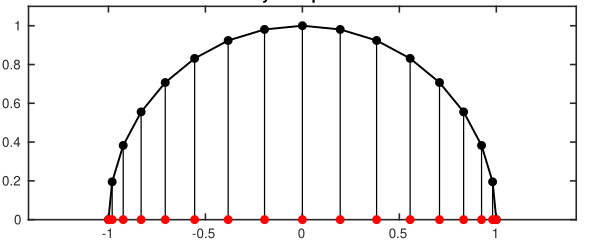
\includegraphics[width=0.8\textwidth]{figures/chebPoints}
	\caption{Точки Чебишева}
\end{figure}

Проєкція цих точок на дійсну вісь дає класичне визначення точок екстремумів поліномів Чебишева другого роду:
\begin{equation}\label{eq:cheb_nodes_def}
	x_j = \cos\left(\frac{j\pi}{n}\right), \qquad 0 \le j \le n.
\end{equation}

Нехай задано набір числових значень $\{f_j\}$, $0 \le j \le n$, які можуть бути отримані шляхом дискретизації певної функції $f(x)$ у вузлах Чебишева. Згідно з базовими положеннями алгебри, існує єдиний інтерполяційний поліном $p(x)$ ступеня не вище $n$, який проходить через ці дані, тобто задовольняє умову $p(x_j) = f_j$ для кожного $j$. Позначимо множину всіх таких поліномів як $\mathcal{P}_n$:
\begin{equation}\label{eq:polynomial_space}
	\mathcal{P}_n = \{ \text{поліноми ступеня не вище } n \}.
\end{equation}

Властивість існування та єдиності поліноміального інтерполянта є справедливою для будь-якого набору попарно різних точок. У специфічному випадку використання вузлів Чебишева отриманий поліном називається \textit{чебишовським інтерполянтом}~\cite{trefethen2013approximation}.

Відомо, що поліноміальні інтерполянти, побудовані на рівномірній сітці точок, мають вкрай погані математичні властивості. Натомість інтерполяція за вузлами Чебишева демонструє відмінну збіжність при слабких вимогах на мінімальну гладкість функції. Фундаментальна різниця між цими підходами полягає у кластеризації точок поблизу кінців інтервалу $1$ та $-1$.

В обчислювальній математиці розрізняють два основні типи чебишовського розподілу: вузли першого роду що э коренями поліномів Чебишева, та вузли другого роду що э точками екстремумів поліномів Чебишева другого роду. Розроблений алгоритм масштабування базується саме на вузлах другого роду.

Головна обчислювальна перевага вузлів другого роду полягає у можливості оптимізації розрахунків при збільшенні порядку інтерполяції. Сітки, побудовані на основі вузлів першого роду, не є вкладеними: при збільшенні порядку полінома, координати абсолютно всіх точок дискретизації змінюються. Це вимагає повного перерахунку значень цільової функції у нових вузлах.

Натомість сітки, що базуються на вузлах Чебишева другого роду, володіють властивістю математичної вкладеності. При подвоєнні кількості інтервалів (перехід від $n$ до $2n$), усі вузли попередньої сітки точно збігаються з парними вузлами нової сітки:
\begin{equation}
	\cos\left(\frac{k\pi}{n}\right) = \cos\left(\frac{2k\pi}{2n}\right).
\end{equation}
Ця алгоритмічна властивість має критичне значення для оптимізації обчислень: при підвищенні точності інтерполяційного процесу не потрібно перераховувати існуючі вузлові значення, необхідно лише обчислити нові значення у проміжних точках.